%=========================================================================
% (c) 2011, 2012 Josef Lusticky <xlusti00@stud.fit.vutbr.cz>

\section{Topology and hierarchy}
As in every other network protocol there are servers and clients.
The servers are rated with the stratum (plural form strata) number which represents their position
in an NTP hierarchy and their possible accurancy~\cite{rfc5905}.
Primary (stratum 1) servers synchronise to the reference clock directly traceable to UTC via
radio, satellite or modem.
The stratum 2 servers synchronise to stratum 1
servers via hierarchical subnet.
The stratum 3 servers synchronise to stratum 2 servers, and so on.
The maximum stratum is 15, number 16 means unsynchronised server
and higher numbers (up to 255) are reserved~\cite{rfc5905}.
Synchronisation between servers in the same stratum level is also possible.
Figure~\ref{fig:ntp-hierarchy} shows a brief hierarchy of NTP.
The clients are always leaves in the NTP hierarchy.
\begin{figure}
  \centering
  %\input{./xfig/test.pstex_t}
  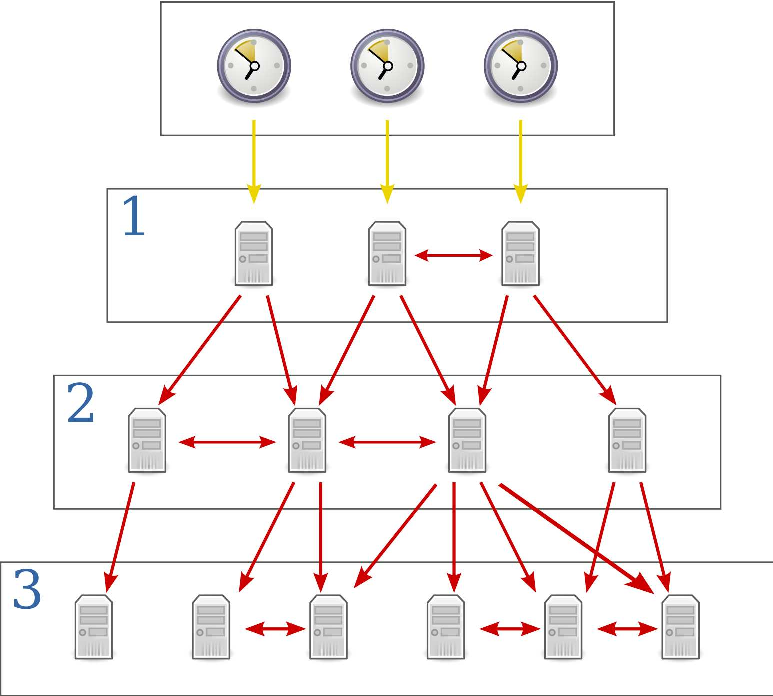
\includegraphics[width=9cm,keepaspectratio]{fig/Network_Time_Protocol_servers_and_clients.pdf}
  \caption{Topology and hierarchy of NTP by B. Esham}
  \label{fig:ntp-hierarchy}
  \bigskip
\end{figure}

